\documentclass[conference]{IEEEtran}
\IEEEoverridecommandlockouts
% The preceding line is only needed to identify funding in the first footnote. If that is unneeded, please comment it out.

\usepackage{cite}
\usepackage{amsmath,amssymb,amsfonts}
\usepackage{algorithmic}
\usepackage{graphicx}
\usepackage{textcomp}
\usepackage{xcolor}
\usepackage{fontspec}
\setmainfont{Times New Roman}
\def\BibTeX{{\rm B\kern-.05em{\sc i\kern-.025em b}\kern-.08em
    T\kern-.1667em\lower.7ex\hbox{E}\kern-.125emX}}
\begin{document}

\title{A Simple Survey of AIGC\\
%{\footnotesize \textsuperscript{*}Note: Sub-titles are not captured in Xplore and
%should not be used}
%\thanks{Identify applicable funding agency here. If none, delete this.}
}

\author{\IEEEauthorblockN{1\textsuperscript{st} Yichi Zhang }\\
\IEEEauthorblockA{\textit{Zhejiang University}\\
Hangzhou, China \\
yichics02@gmail.com}
}

\maketitle

\begin{abstract}
AIGC refers to Artificial Intelligence Generated Content, 
which is generated automatically or collaboratively using 
artificial intelligence techniques in response to user input 
or demand, including text, images, audio, video, and other forms 
of content. In this survey, the basic principles of Transformer 
and diffusion models are presented. The GPT and BERT models 
based on Transformer are introduced, as well as three different 
types of diffusion models and their practical applications. 
Finally, the security and robustness issues of AIGC models are 
discussed.
\end{abstract}

\begin{IEEEkeywords}
AIGC, Transformer, Diffusion, Security, Robustness
\end{IEEEkeywords}

\section{Introduction}
This survey will cover the following contains: First , 
we will focus on explaining the basic principles of the Transformer, 
followed by a discussion of the details of language models (LLMs) 
that use the Transformer, such as BERT, GPT, etc. 
We will also cover some techniques for training and optimizing 
these models. 
Finally, we will discuss the security and 
robustness of GPT models, respectively, 
based on recent research findings.

\section{Transformer}
\par Generative models have a long history in artificial intelligence, dating back to the 1950s with the
development of Hidden Markov Models (HMMs) [20] and Gaussian Mixture Models (GMMs) [21 ].
These models generated sequential data such as speech and time series. However, it wasn’t until
the advent of deep learning that generative models saw significant improvements in performance.
In early years of deep generative models, different areas do not have much overlap in general.
In natural language processing (NLP), a traditional method to generate sentences is to learn
word distribution using N-gram language modeling [22] and then search for the best sequence.
However, this method cannot effectively adapt to long sentences. To solve this problem, recurrent
neural networks (RNNs) [23] were later introduced for language modeling tasks, allowing for
modeling relatively long dependency. This was followed by the development of Long Short-Term
Memory (LSTM) [ 24 ] and Gated Recurrent Unit (GRU) [ 25 ], which leveraged gating mechanism to
control memory during training. These methods are capable of attending to around 200 tokens in a
sample [26], which marks a significant improvement compared to N-gram language models.

\par Meanwhile, in computer vision (CV), before the advent of deep learning-based methods, tra-
ditional image generation algorithms used techniques such as texture synthesis [27] and texture
mapping [28]. These algorithms were based on hand-designed features, and were limited in their abil-
ity to generate complex and diverse images. In 2014, Generative Adversarial Networks (GANs) [ 29]
was first proposed, which was a significant milestone in this area, due to its impressive results
in various applications. Variational Autoencoders (VAEs) [30] and other methods like diffusion
generative models [31] have also been developed for more fine-grained control over the image
generation process and the ability to generate high-quality images.
\par The advancement of generative models in various domains has followed different paths, but
eventually, the intersection emerged: the transformer architecture [32]. The Transformer was 
initially developed to handle NLP tasks, but it has also been applied to tasks in computer vision. 
Its various variants for different tasks quickly achieved state-of-the-art performance. In the field of NLP, many
prominent large language models, e.g., BERT and GPT, adopt the transformer architecture as
their primary building block. In CV, Vision Transformer (ViT) [ 35 ] and Swin Transformer [ 36] 
later takes this concept even further by combining the transformer architecture with visual components, 
allowing it to be applied to image based downstreams. 
Except for the improvement that transformer brought
to individual modalities, this intersection also enabled models from different domains to be fused
together for multimodal tasks. One such example of multimodal models is CLIP [ 37 ]. CLIP is a
joint vision-language model that combines the transformer architecture with visual components,
allowing it to be trained on a massive amount of text and image data. Since it combines visual
and language knowledge during pre-training, it can also be used as image encoders in multimodal
prompting for generation. In all, the emergence of transformer based models revolutionized AI
generation and led to the possibility of large-scale training.

\subsection{Model Architecture of Transformer}
\par Here is a diagram of the Transformer model architecture. 
We will now explain this architecture by focusing on several modules: 
Encoder-Decoder, Self-Attention, Position-wise Feed-Forward Network, 
Embeddings, and Softmax.

\begin{figure}[htbp]
    \centerline{
\includegraphics[width = 8cm]{pic/fig1.png}}
    \caption{Model Architecture of Transformer}
    \label{fig}
\end{figure}

\subsubsection{Encoder-Decoder}

\par The Encoder consists of $N$ layers, each of which contains two sub-layers. 
The first sub-layer includes a Multi-Head Attention module, and the 
second sub-layer includes a position-wise fully connected feed-forward network. 
In each sub-layer, we apply a residual connection module, followed by layer normalization.

\par The Decoder also consists of $N$ independent layers, but unlike the Encoder, 
each layer of the Decoder contains three sub-layers, which has three different kinds of modules: 
Masked Multi-Head Attention, Multi-Head Attention, and position-wise fully connected 
feed-forward network. Similarly, we apply the same residual connection and layer 
normalization after each sub-layer.

\par This results in the following equation for each sub-layer:
\begin{align*}
    Output(x) = LayerNorm(x + SubLayer(x))
\end{align*}

where $Sublayer(x)$ is the function implemented by the sub-layer itself.


\subsubsection{Attention}
\par An attention function can be described as mapping a query and a key-value pair 
to a set of outputs, where all of these quantities are vectors. This allows the output 
to be viewed as a weighted sum of values, where each value's weight can be seen as 
calculated based on the query and its corresponding key.

\begin{figure}[htbp]
    \centerline{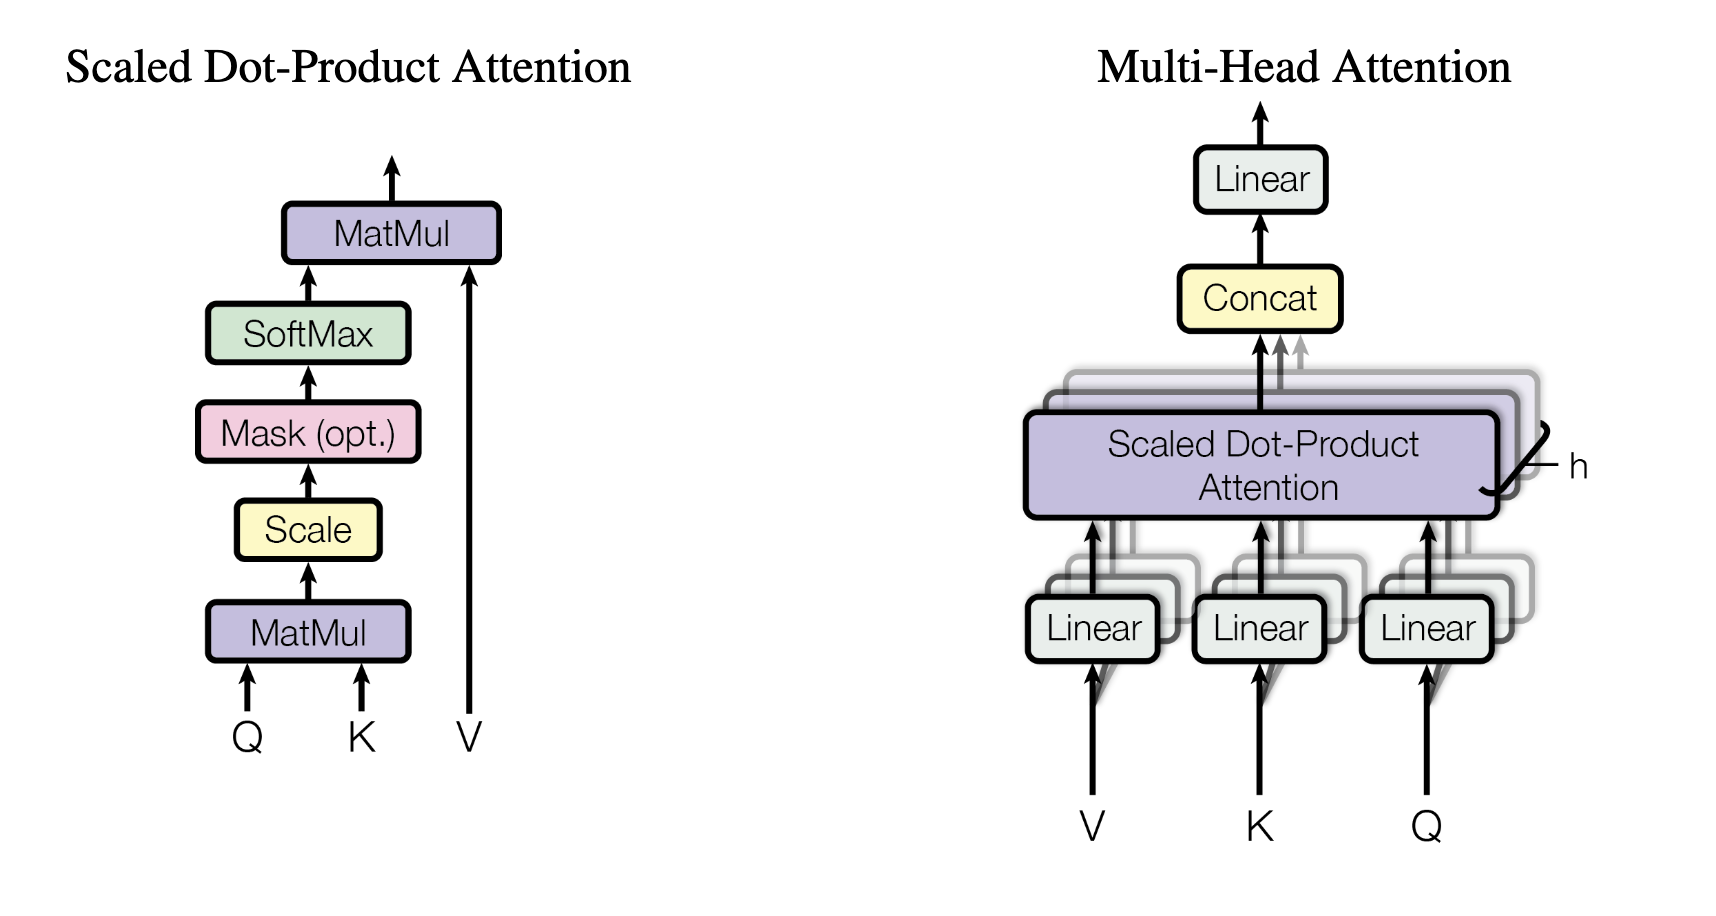
\includegraphics[width = 8cm]{pic/fig2.png}}
    \caption{Attention Mechanism}
    \label{fig}
\end{figure}

\par From Fig2, we can see that the Multi-Head Attention used in the model consists of 
multiple Scaled Dot-Product Attention modules. Therefore, let's focus on 
Scaled Dot-Product Attention first.
\begin{align*}
    Attention(Q, K, V) = softmax(\frac{QK^T}{\sqrt{d_k}})V
\end{align*}

\par Compared to regular dot-product attention, Scaled Dot-Product Attention includes a 
scaling factor $\sqrt{d_k}$ in the equation to improve the performance of the softmax 
function on larger datasets.

\par Next, let's consider how to apply Scaled Dot-Product Attention to Multi-Head Attention. 
For a set of $K$, $Q$, $V$, each with a $d_{model}$ dimension, they are projected to different 
dimensions ($d_k$, $d_k$, and $d_v$, respectively). Then, attention calculations are 
performed in parallel on the projected versions of the $Q$, $K$, and $V$, 
resulting in an output vector with a dimension of $d_v$.
\begin{align*}
    MultiHead&(Q, K, V) = Concat(head_1, head_2, ... , head_h)W^O \\
    where \  &head_i = Attention(QW^Q_i, KW^K_i, VW^V_i)\\
    &W^Q_i \in \mathbb{R}^{d_{model}\times d_k}, \  
    W^K_i \in \mathbb{R}^{d_{model}\times d_k}\\
    &W^V_i \in \mathbb{R}^{d_{model}\times d_v}, \ 
    W^O \in \mathbb{R}^{hd_v \times d_{model}}
\end{align*}

\par Where $h$ is the number of attention layers that are computing in parallel.

\par Note that in Fig2, there is also an optional mask module used to mask out certain 
invalid positions or information when calculating attention scores. This is done 
to prevent these invalid positions or information from being considered when calculating 
attention weights.

\subsubsection{Position-wise Feed-Forward Networks}

\par In each layer of the Encoder or the Decoder, there is a fully connected feed-forward 
network that is applied  separately and identically to each position. This network consists of 
two layers of ReLU activation functions combined together.
\begin{align*}
    FFN(x) = max(0, xW_1 + b_1)W_2 + b_2
\end{align*}

\par Of course, different layers may use different parameters, and there may be changes 
in dimensions caused by modules such as convolutional layers between layers.

\subsubsection{Embeddings and Softmax}

\par Like other sequence processing models, the Transformer also uses a learnable 
embedding to convert input and output tokens into $d_{model}$-dimensional vectors. It also 
uses a learnable linear transformer and softmax function to convert the decoder's output 
into predicted probabilities for the next token.In the embedding layers, 
multiply those weights by $\sqrt{d_{model}}$.

\subsubsection{Positional Encoding}

\par Since the Transformer does not contain convolutional or recurrent components, 
position encoding is required to incorporate positional information of the input sequence. 
Here, the position encoding uses the same dimension as the embedding to enable addition of the two. 
Given that there are various forms of position encoding, both learnable and fixed, 
the Transformer uses sine and cosine functions of different frequencies to encode position information.

\begin{align*}
    PE_{(pos,2i)} &= \sin(pos/10000^{2i/d_{model}})\\
    PE_{(pos,2i+1)} &= \cos(pos/10000^{2i/d_{model}})
\end{align*}

\par where $pos$ is the position and $i$ is the dimension.


\subsection{Training of Transformer}
\par In the original Transformer paper, the model was trained on the standard WMT 2014 English-German 
dataset using the Adam optimizer with hyperparameters $\beta_1 = 0.9$, $\beta_2 = 0.98$, and 
$ \epsilon = 10^{-9}$. The learning rate was assigned based on a formula, where the number 
of $warmup\_steps$ was set to 4000.

\begin{align*}
    lrate = \frac{min({step\_num}^{0.5}, step\_num \cdot warmup\_steps^{-1.5})}{\sqrt{d_{model}}}
\end{align*}

\par In addition, to prevent overfitting during training, several regularization 
techniques were applied, such as Residual Dropout with $P_{drop} = 0.1$ and label 
smoothing with a value of $\epsilon_{ps} = 0.1$. The use of these techniques allowed 
the Transformer to achieve better performance after training.

\section{BERT}

\par BERT, which stands for Bidirectional Encoder Representations fromTransformers. 
Unlike recent language representation models (Peters et al., 2018a; Radford et al., 2018), 
BERT is designed to pre-train deep bidirectional representations from
unlabeled text by jointly conditioning on both left and right context in all layers. As a 
result, the pre-trained BERT model can be fine-tuned with just one additional output layer
to create state-of-the-art models for a wide range of tasks, such as question answering and
language inference, without substantial taskspecific architecture modifications.

\subsection{Model Architecture of BERT}
\par The model architecture of BERT is a multi-layer bidirectional Transformer encoder 
based on the Transformer architecture. Compared to the original Transformer architecture, 
BERT uses a bidirectional structure, which will be explained in more details later.

\par In addition, BERT also employs different structures for input and output 
representations. To adapt to different downstream tasks, the input representation 
should be able to handle sequences consisting of multiple sentences as single token. 
Therefore, BERT uses WordPiece embeddings for this purpose.

\par In BERT, the first token of each sequence is a special classification token ([CLS]). 
Sentences pairs are packed into a single sequence. There are two methods to differentiate 
between different sentences within a sequence. Firstly, a special separator token ([SEP]) 
is used to separate different sentences. Secondly, a learnable embedding is added to each 
token to indicate which sentence it belongs to.For a given token, its input representation 
is constructed by summing the corresponding token, segment, and position embeddings, that's 
what Fig3 shows.

\begin{figure}[htbp]
    \centerline{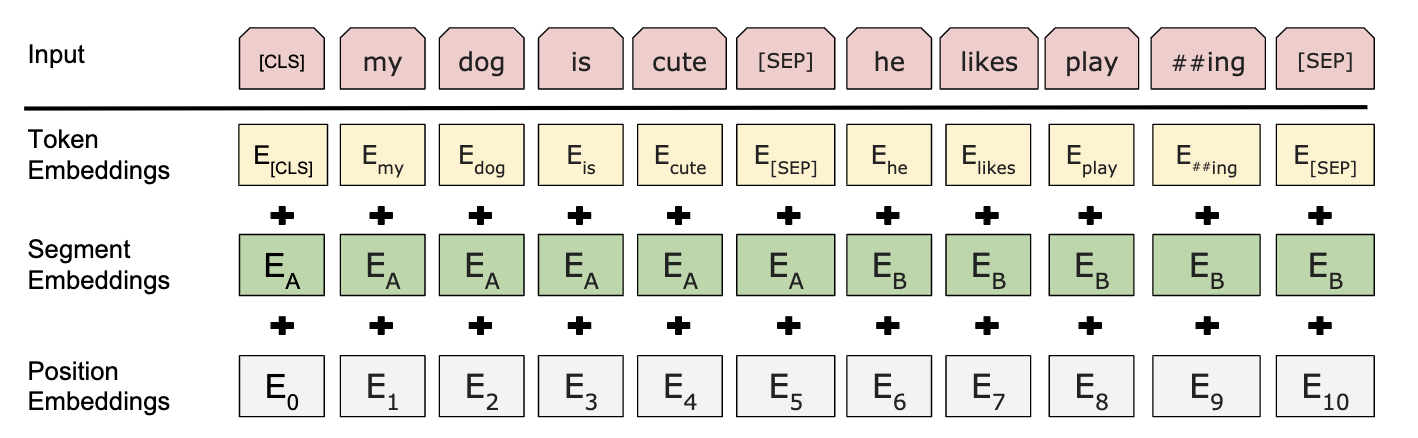
\includegraphics[width = 8cm]{pic/fig3.png}}
    \caption{Input Representation of BERT}
    \label{fig}
\end{figure}


\subsection{Training of BERT}

\par Training BERT is a crucial part of its development, and it involves several 
techniques, including Unsupervised Feature-based Approaches, Unsupervised 
Fine-tuning Approaches, and Transfer Learning from Supervised Data. The training 
process is divided into two parts. 

\begin{figure}[htbp]
    \centerline{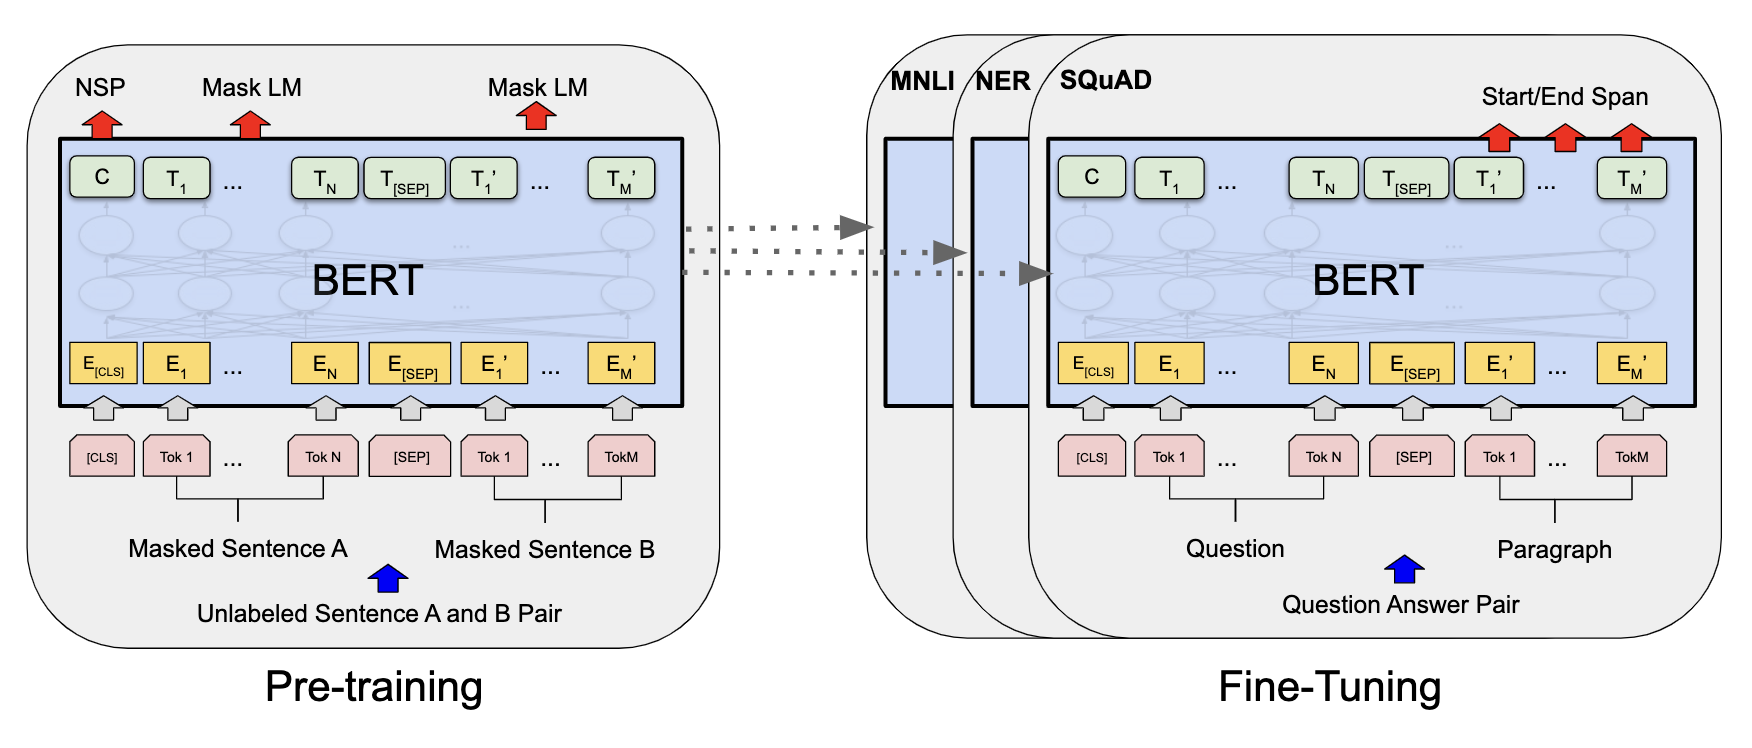
\includegraphics[width = 8cm]{pic/fig4.png}}
    \caption{Training of BERT}
    \label{fig}
\end{figure}

\par The first part is Pre-Training, during which BERT 
is trained to perform two tasks.Task 1 is Masked Language Modeling (MLM), where 
15\% of the wordpiece tokens are randomly masked and replaced with a special token ([MASK]). 
BERT is then trained to predict these masked tokens.Task 2 is Next Sentence Prediction (NSP), 
where BERT is given a pair of sentences A and B and is trained to predict whether 
sentence B follows sentence A.

\par The second part is fine-tuning, where we use a small amount of 
labeled data to train BERT for specific downstream tasks. Because of the properties of 
the Transformer architecture, BERT can model downstream tasks by adjusting its inputs and 
outputs. During fine-tuning, BERT uses bidirectional self-attention mechanisms to encode 
text and to coordinate and unify its inputs and outputs for the specific task at hand.

\section{GPT}

\par GPT (Generative Pre-trained Transformer) is a Transformer-based pre-trained language 
model developed by OpenAI. The development of GPT can be divided into four versions. 
GPT-1 was pre-trained on a large corpus of text and was one of the first models to 
demonstrate excellent performance in natural language processing tasks. GPT-2 is an 
improved version of GPT-1, pre-trained on larger datasets with more parameters, and 
can generate more natural and fluent text. GPT-3 is a much larger pre-trained language 
model with 175 billion parameters, achieving state-of-the-art results on various natural 
language processing tasks. As of today, GPT-4 is currently under development, expected 
to have even larger model parameters and better support for multimodal input to handle 
more complex tasks.

\subsection{GPT-1}

\par GPT-1 implemented a semi-supervised approach that combines unsupervised pre-training 
and supervised fine-tuning to accomplish language understanding tasks. This approach 
enables a large amount of training to form a global transformation, and only minor 
adjustments are needed to adapt to a wide range of downstream tasks.

\subsubsection{Model Architecture of GPT-1}

\par GPT-1 uses a TransformerDecoder as its primary architecture, 
which has been proven to have strong performance on various tasks. However, 
depending on the specific task, we can replace or fine-tune different modules 
of the model, such as its input and output, to better adapt to the task at hand.

\begin{figure}[htbp]
    \centerline{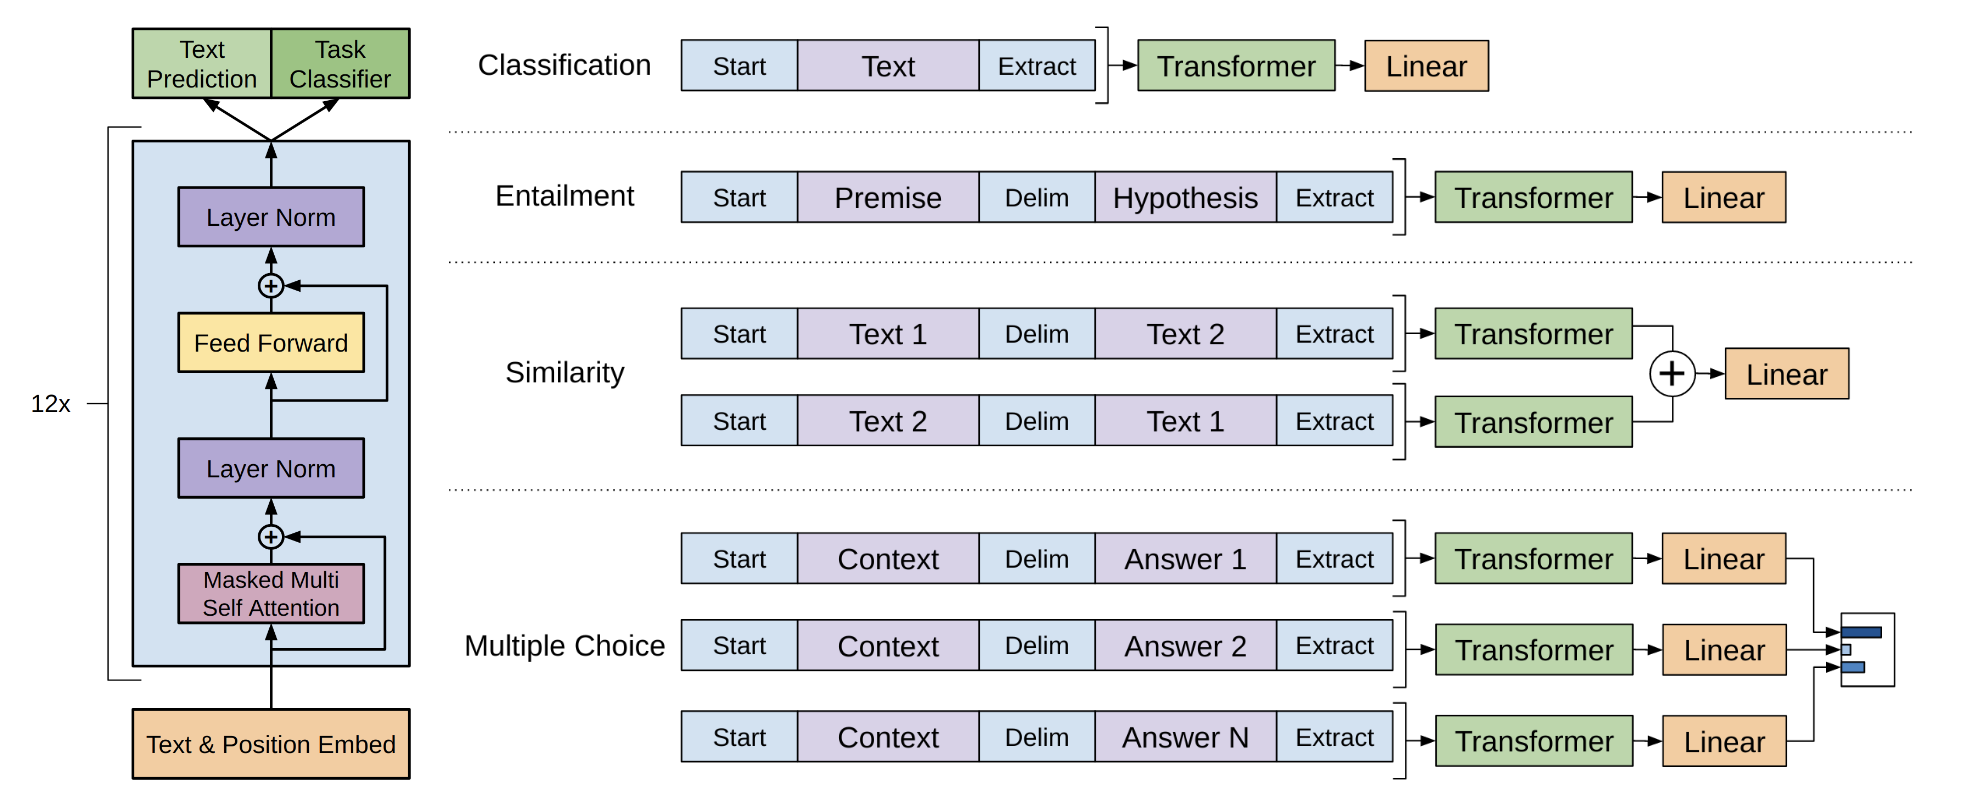
\includegraphics[width = 8cm]{pic/fig5.png}}
    \caption{Model Architecture of GPT-1 \& The Task-specific for different tasks}
    \label{fig}
\end{figure}

\par As GPT use a Transformer Decoder, this model applies multi-headed self-attention 
operation over the input context tokens, followed by position-wise feedforward layers, 
to produce an output distribution over target tokens.

\begin{align*}
    h_0 &= UW_e + W_p \\
    h_l &= transformer\_block(h_{l-1})\ \forall i \in \left[1, n\right] \\
    P(u) &= softmax(h_n W_e^T)
\end{align*}

\par where $U = (u_{-k}, ..., u_{-1})$ is the context vector of tokens, $n$ is the number of layers, 
$W_e$ is the token embedding matrix, and $W_p$ is the position embedding matrix.

\subsubsection{Training of GPT-1}

\par The training of GPT-1 is divided into two parts.

\par The first part being unsupervised pre-training.In this process, GPT is given a 
set of unlabeled corpus tokens $\mathcal{U} = \{u_1, u_2, ..., u_n \}$ and utilizes a standard language model to maximize 
the following likelihood:

\begin{align*}
    L_1(\mathcal{U}) = \sum_{i}\log P(u_i | u_{i-k}, ..., u_{i-1};\Theta )
\end{align*}

\par where $k$ is the size of the context window, and the conditional probability $P$ is 
modeled using a neural network with parameters $\Theta$. These parameters are trained 
using stochastic gradient descent [51].

The second part is supervised fine-tuning, which involves adjusting the model parameters 
for a specific task after unsupervised pre-training. Assuming there is a labeled 
dataset $\mathcal{C} $, where each input has an associated label. The input is processed by the 
model to obtain an activation value $h^m_l$, which, when multiplied by $W_y$, can predict the 
label $y$. This allows us to maximize the following objective $L_2(\mathcal{C})$:

\begin{align*}
    P(y | x^1, x^2, ..., x^m) &= softmax(h_l^m W_y) \\
    L_2(\mathcal{C}) &= \sum_{i}\log P(y | x^1, x^2, ..., x^m)
\end{align*}

Adding a language model as an auxiliary objective during supervised fine-tuning 
can improve learning by (a) enhancing the generalization ability of the supervised 
model, and (b) accelerating convergence. Therefore, we perform a maximization operation 
on the following objective $L_3(\mathcal{C})$:

\begin{align*}
    L_3(\mathcal{C}) = L_2(\mathcal{C}) + \lambda L_1(\mathcal{C})
\end{align*}

\par where $\lambda$ is weight.

\subsection{GPT-2}

\par GPT-2 largely follows the architecture of its predecessor GPT-1, 
with only minor modifications. Layer normalization is moved to after the input 
of each sub-block, and additional layer normalization is added after the final 
self-attention module. A modified initialization is used to account for accumulation 
on the residual path with model depth, where the weights of residual layers are scaled 
by a factor of $1/\sqrt{N}$ at initialization, with $N$ being the number of residual layers. 
The vocabulary is expanded to 50,257, and the context size is increased from 512 to 
1024 tokens. A larger batch size of 512 is also used.

\par GPT-2 was trained on the WebText dataset, and in the original paper, 
the authors evaluated GPT-2's performance on various tasks, including Language Modeling, 
Children's book test, LAMBADA, Winograd Schema Challenge, Reading Comprehension, 
Translation, and Question Answering. As the number of parameters increased, 
GPT-2 exhibited remarkable abilities.

\subsection{GPT3}

\par The model size and amount of data used for training in GPT-3 have significantly 
increased. GPT-3 has 96 layers, each with 96 attention heads, for a total of 175 billion 
parameters, which is 116 times more than GPT-2. GPT-3 was trained on a 45 terabytes 
text dataset selected from Common Crawl, containing 500 billion words, which is 
10 times larger than the dataset used for GPT-2.

\par GPT-3's main selling point is few-shot learning, which means it can complete various 
downstream tasks with only a few examples as input, without fine-tuning or gradient 
updates. GPT-3 has demonstrated outstanding performance on several natural language 
processing tasks, even surpassing some specially designed models.

\subsection{GPT4}

\par GPT-4's main selling point is multimodal learning, which means it 
can accept both images and text as input, and output text. 
GPT-4 can generate descriptive or creative text based on the content 
of the images, and it can also generate relevant images based on the content 
of the text. 


%\section{Diffusion Model}
%\subsection{Foundations of Diffusion Models}
%\subsection{Applications of Diffusion Models}
%\subsection{Optimizing}

\section{Security and Robustness of GPT}








\begin{thebibliography}{00}
\bibitem{b1} G. Eason, B. Noble, and I. N. Sneddon, ``On certain integrals of Lipschitz-Hankel type involving products of Bessel functions,'' Phil. Trans. Roy. Soc. London, vol. A247, pp. 529--551, April 1955.
\bibitem{b2} J. Clerk Maxwell, A Treatise on Electricity and Magnetism, 3rd ed., vol. 2. Oxford: Clarendon, 1892, pp.68--73.
\bibitem{b3} I. S. Jacobs and C. P. Bean, ``Fine particles, thin films and exchange anisotropy,'' in Magnetism, vol. III, G. T. Rado and H. Suhl, Eds. New York: Academic, 1963, pp. 271--350.
\bibitem{b4} K. Elissa, ``Title of paper if known,'' unpublished.
\bibitem{b5} R. Nicole, ``Title of paper with only first word capitalized,'' J. Name Stand. Abbrev., in press.
\bibitem{b6} Y. Yorozu, M. Hirano, K. Oka, and Y. Tagawa, ``Electron spectroscopy studies on magneto-optical media and plastic substrate interface,'' IEEE Transl. J. Magn. Japan, vol. 2, pp. 740--741, August 1987 [Digests 9th Annual Conf. Magnetics Japan, p. 301, 1982].
\bibitem{b7} M. Young, The Technical Writer's Handbook. Mill Valley, CA: University Science, 1989.
\end{thebibliography}
\vspace{12pt}

\end{document}
